
\chapter{Introduction}
\label{Chap:Intro}

\setcounter{section}{-1}

\section{Let there be Light}

``\textit{God said, `Let there be light,' and there was light. God saw that the light was good, and he separated the light from the darkness. God called the light `day,' and the darkness he called `night'. And there was evening, and there was morning — the first day.}'' \textasciitilde Genesis 1:3-5.

Since the dawn of life itself, we have been exposed to the natural light of the sun, and the distinct separation of day and night. However, our modern, fast-paced lifestyle no longer allows for such long periods of time being wasted and unproductive in darkness.

As the literature reveals more and more ways in which this divergence harms our well-being, it seems that a serious re-think of our environments - and how we light them - is required.

\section{Gap in the Market}

Light has been shown to have serious ramifications on many facets of life: excess \gls{BlueLight} in the evenings causing sleep deficiency; lighting affecting lifestyle-related diseases; insufficient \gls{BlueLight} exposure being a risk factor for depression and other mood disorders; and plenty more that are discussed in chapter \ref{Chap:Lit}.

Chapter \ref{Lit:solutions} outlines why the existing products attempting to solve this problem are not appropriate, and thus why a new solution must be developed. 

\section{Aims and Objectives}

This project set out to try to develop an affordable, modular, broad-application natural lighting solution. 

\subsection{Aims}

There were 2 main aims that the device set out to achieve: 'To produce an affordable device that replicates the visual solar spectrum as closely as is feasible' and 'to validate the device by measuring the output spectra across the day'.

Initially, further aims included developing the device as a product by improving user experience through user interface, web apps, and other expanded functionality. This would have been researched using qualitative methods such as opinion surveys to assess the interest in the device in the consumer market. These aims were set out as stretch goals that could be undertaken when the two main aims had been completed.

\subsection{Objectives}

\begin{figure*}[bt]
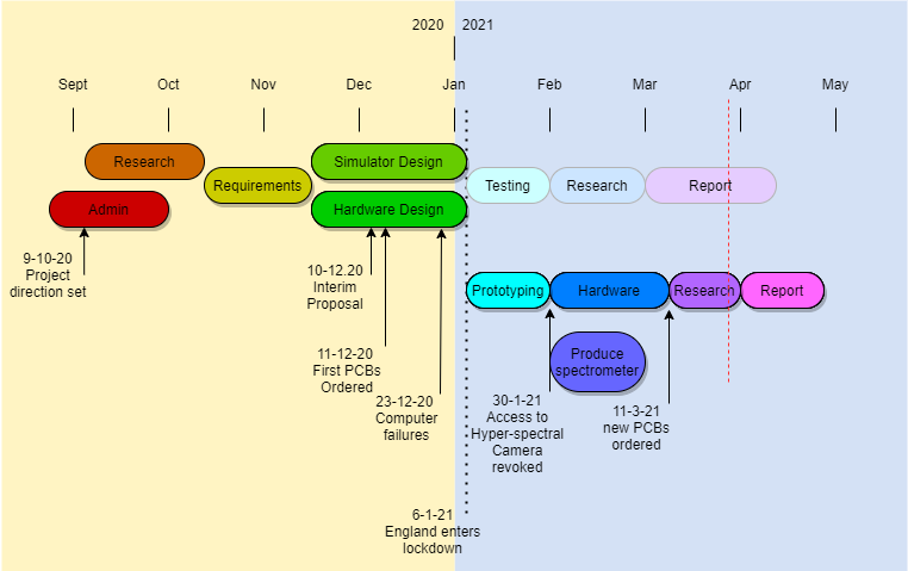
\includegraphics[width=\textwidth]{Images/plan}
\caption{How the lockdown in England affected the objectives of the project. Reasons for the changes are discussed later in the document.}
\label{Objectives}
\end{figure*}

The objectives used to achieve the aims have been dynamic throughout the project. The initial plan of producing and testing 2 rounds of \acrfull{pcbs} before using these to validate the spectral outputs was heavily influenced by the pandemic. See Fig \ref{Objectives}.

Both N. Appleton and V. Halenka were involved in the design of the hardware, as it was a useful device for both areas of research. The success of these devices was assessed against the requirements specification (Appendix \ref{App:Req} and is discussed in chapter (REF).

One of the most important aims of the project from the beginning was the development of the simulator. This allowed for a contingency for that spectral measurements to be obtained even in the absence of physical hardware. The simulator was also used to explore the desired outputs of the device and how they could be achieved.

\subsection{Scope}

Keeping the scope of the project relatively flexible was an important factor due to the pandemic. Designing the hardware, which was scheduled to be done by February, was severely impacted by the lockdown that began on the 1st of January 2021. 

Due to the ``modular'' construction of the aims, the qualitative, product-based research and much of the usability development had to be left for future research and development. In removing these aims from the project, it allowed the primary objective to be successfully achieved.

Had the pandemic not had such a profound effect, the main aims would have likely been completed earlier, allowing for progression to the secondary research goals. However, going into the project, there was no way to know how the year would pan out. Using this dynamic scope worked very well and allowed the successful completion of the primary area of research. 



\section{Project Management}

%This project was approached in a self-led manner, with the hardware design being split across 2 projects. Weekly supervisor meetings have been held as well as meetings between N. Appleton and V. Halenka to ensure that all areas of work are on schedule.

\paragraph{AGILE Kanban}

The project was approached using a Kanban-style AGILE workflow, using the $ClickUp^{TM}$ project management software to organise tasks, subtasks, Gantt charts, meeting minutes, relevant literature and more. Using just one piece of software to organise all of this reduced the friction and chance of errors. For example, when updating Gantt charts, the Kanban boards and tasks are automatically updated to reflect these changes and vice versa.

\paragraph{Weekly meetings}
Both weekly supervisor meetings, and weekly meetings between the hardware developers took place to ensure that all areas of the project were progressing as planned. Alterations to the scheduled work could be discussed and approved at these meetings, further reducing the friction when needing feedback. Minutes of these meetings were made on the $ClickUp^{TM}$ software and copies were printed and pasted into the project logbook.

\paragraph{Logbook}
The logbook has been used as a hard-copy of all the digital documents that were produced throughout the project including interviews, requirements documentation, meeting minutes, invoices, design documentation and Gantt charts. All work has been logged to ensure data is not lost and the project could continue even in the event of the researcher being replaced. 

\paragraph{Gantt Charts}
The project plan Gantt charts were updated on a monthly basis to ensure their relevance and to take into account the most up-to-date information. These updates happened in meetings between the development team to allow timescales to be discussed before implementation. All Gantt charts are displayed in appendix \ref{App:Gantt}.

\paragraph{Time Constraints}
As with any project, there have been some strictly imposed time constraints throughout the year. Weekly supervisor meetings meant that there was always a two-way stream of information so as to put less importance on each meeting. 

It was important that the experimentation could be completed by the end date of the project, and that at least initial results could be gathered before the progress review that took place at the end of March.

\paragraph{Contingencies}
From the beginning of the project, a focus has been placed on creating effective contingencies to ensure that the main experimentations would give results. This has been especially true within a hardware-based project during the pandemic. The flexible aims have been discussed earlier, but many other contingencies were put in place. Building a simulator was a big priority to ensure that results could be gathered in the event of failure to obtain hardware.

\paragraph{Risks and Mitigation}
The project has been focused on de-risking throughout by front-loading the highest-risk tasks to ensure that, in the case of failure, objectives can still be met. For example, hardware development happened early on in the project to allow time to overcome any of the issues that arose.

This method of risk identification and mitigation proved extremely effective during the pandemic, when many of the unwanted outcomes came to pass.

The risk-assessment and resources forms have been kept up-to-date throughout the project to ensure that a safe working environment can be guaranteed. Few changes were made to these documents as the initial copies were good reflections of the risks and resources required.

\paragraph{Reflection}
The successful completion of all the main outcomes of the project is a testament to the good planning that has been observed from the beginning.

The continued planning  and de-risking, alongside the effective use of supervision, have ensured that all the primary aims were achieved within the timeframe. This, in turn, allowed the adherence to milestones and deadlines, including the progress review. Contingencies played a large role in delivery of the project, and are discussed further in chapter \ref{Sec:physicalOuts}.

Mitigating any potential risks through the use of the risk-assessment (Appendix \ref{App:Risk} early in the project allowed for progress to be made safely and appropriately. 

The Engineering Council's UK-SPEC has been consulted throughout the project and a spreadsheet has been kept up to date containing relevant evidence of each competency. This has helped to keep the project relevant to engineering professionalism and personal development. The logbook has been used as the main repository for all of the relevant documentation, minutes, notes and technical details. Using this, alongside $ClickUp^{TM}$ for planning tasks and time management, has streamlined the workflow, allowing for much more efficient use of time.

Overall, the management of this project has been executed excellently and, despite the pandemic, all changes to circumstance have been overcome (more in chapter \ref{Sec:physicalOuts}).

% UK SPEC


